The frozen prospective candidate experiment evaluates 128 new paired artificial worlds, each containing 24 candidates. The old loose screen buys 1,412 unreachable assessments; the reachability-first rule buys 0. Mean modeled net improvement is \$22.05 per world, with conditional Monte Carlo 95\% interval [\$21.24, \$22.85]. Admission counts match in all 128 worlds. Each rule still makes 25 modeled false admissions. Reachability removes a logical impossibility; it does not solve imperfect assessment or establish an expertise gain.
\begin{figure}[H]\centering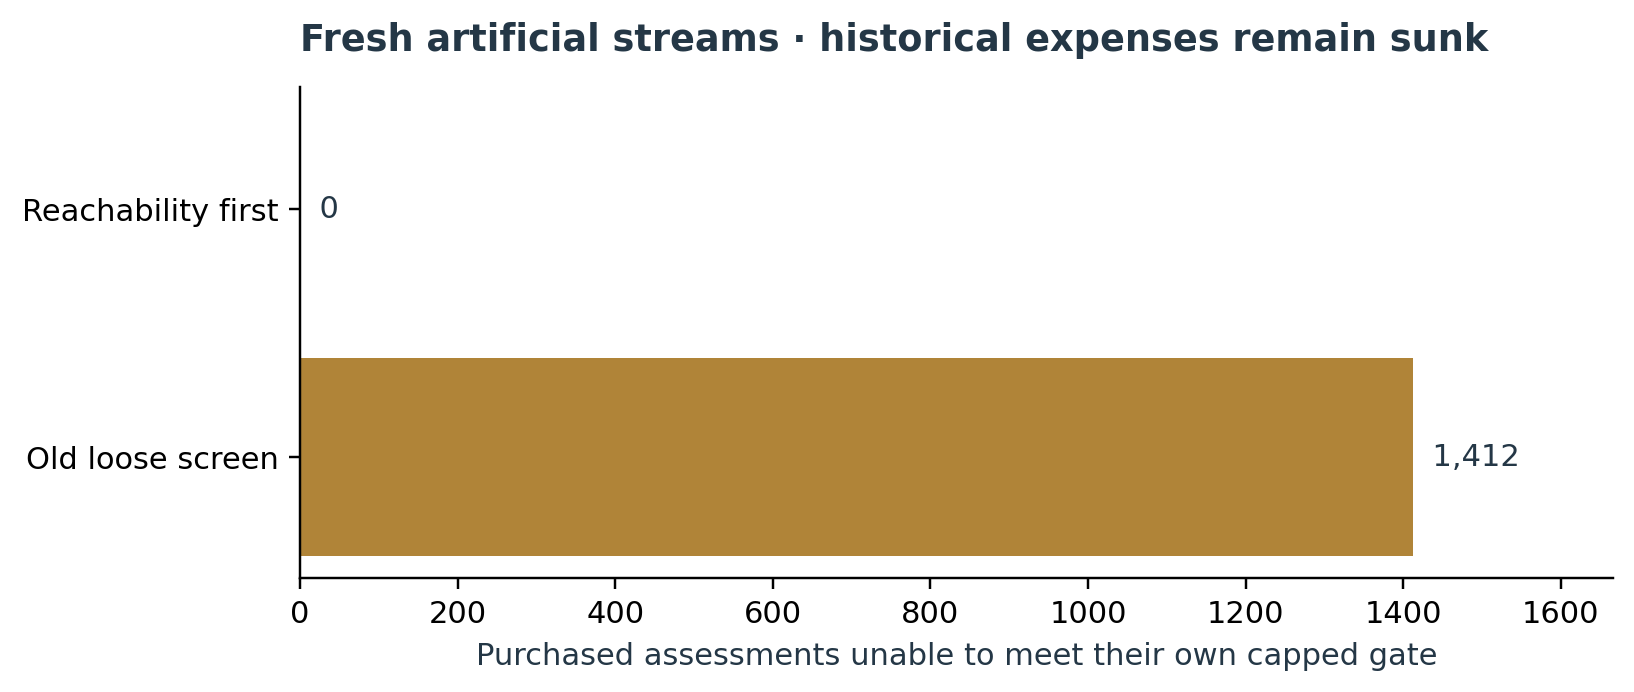
\includegraphics[width=0.95\linewidth]{figures/admission_reachability.png}\caption{Separate prospective synthetic controller comparison. All costs and benefits are modeled; no historical assessment is refunded or erased.}\end{figure}
